\taskpic{ В цилиндрическом сосуде с водой плавает кусок льда объёмом
  $V_0 = 1000$~см$^3$.  В лёд вморожена свинцовая пуля объемом $V_1 =
  1$~см$^3$. Ко льду на невесомой нерастяжимой нити привязан воздушный
  шарик, заполненный гелием. Оболочка шарика имеет пренебрежимо малую
  массу. Каким должен быть объём шарика $V$, чтобы после таяния льда
  уровень воды в сосуде не изменился? Необходимые справочные данные
  приведены ниже: плотность гелия $\rho_{\mbox{гел.}} =
  0{,}2$~кг/м$^3$; плотность воздуха $\rho_{\mbox{возд.}} =
  1{,}3$~кг/м$^3$; плотность льда $\rho_{\mbox{льда}} =
  0{,}9$~г/см$^3$; плотность воды $\rho_{\mbox{воды}} = 1$~г/см$^3$;
  плотность свинца $\rho_{\mbox{свинца}} = 11{,}3$~г/см$^3$.  }
{
  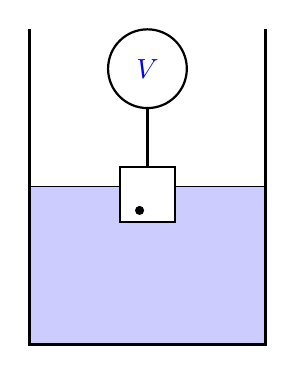
\begin{tikzpicture}
    \draw[thin,fill=blue!20] (0,0) rectangle (3,2);
    \draw[very thick] (0,4) -- (0,0) -- (3,0) -- (3,4);
    \draw[thick,fill=white] (1.15,1.55) rectangle (1.85,2.25);
    \draw[thick] (1.5,2.25) -- (1.5,3);
    \draw[thick] (1.5,3.5) circle (0.5) node[blue] {$V$};
    \draw[fill=black] (1.4,1.7) circle (0.05cm);
  \end{tikzpicture}
}
% Город-2007, 7 класс
